\chapter{Аналитическая часть}

В данном разделе будут рассмотерны существующие решения и проведен их анализ, 
сформулированы требования к разрабатываемой 
базе данных, проведен анализ существующих баз данных, а также описаны
пользователи системы.

\section{Существующие решения}

Так как IoT-вещей активно развиваются, то на рынке уже представлены различные платформы умных домов. 
Рассмотрим наиболее популярные из них:
\begin{itemize}
    \item Apple Homekit~\cite{apple}
    \item Intel IoT Platform~\cite{intel}
    \item MTS IoT HUB~\cite{mts}
    \item Xiaomi MI~\cite{xmi}
\end{itemize}

Выделим следующие критерии для сравнения выбранных платформ:
\begin{enumerate}
    \item[1)] Многопользовательский доступ
    \item[2)] Возможность создания нескольких домов
    \item[3)] История работы устройств
\end{enumerate}

Сравнение выбранных платформ по указанным критериям представлены в таблице \ref{tab:solutions}:
\begin{table}[!ht]
    \centering
    \caption{\label{tab:solutions} Сравнение существующих решений}
    \begin{tabular}{|l|l|l|l|l|l|}
    \hline
        Решение & 1 & 2 & 3  \\ \hline
        Apple Homekit & + & + & - \\ \hline
        Intel IoT Platform & - & - & + \\ \hline
        MTS IoT HUB & - & + & + \\ \hline
        Предполагаемое решение & + & + & + \\ \hline
    \end{tabular}
\end{table}

Таким образом, ни одна из плафторм не удовлетворяет всем критериям. 

\section{Формулирвока требований к разрабатываемой базе данных и приложению}

В ходе выполнения курсовой работы необходимо разработать базу данных для хранения информации 
о пользователях, умных домах, устройствах. 

Помимо этого, нужно спроектировать Web-приложение, 
которое будет предоставлять интерфейс для взаимодействия с базой данных с возможностью создавать умные дома, 
добавлять новые устройтва в свой дом, просматривать историю работы устройств.
    
Необходимо также предусмотреть многопользовательский доступ к дому, возможность добавления других пользователей 
в свой дом для совместного управления. Требуется реализовать функциональность для разных категорий пользователей, 
каждый из которых получает свой определенный набор прав.

\section{Формализация данных}

Разрабатываемая база данных для IoT платформы умного дома должна содержать информаицю о пользователях, устройствах, умных домах,
истории работы устройств. Данные категории показаны на ER-диаграмме в нотации Чена \ref{img:er}.

\begin{figure}[h]
    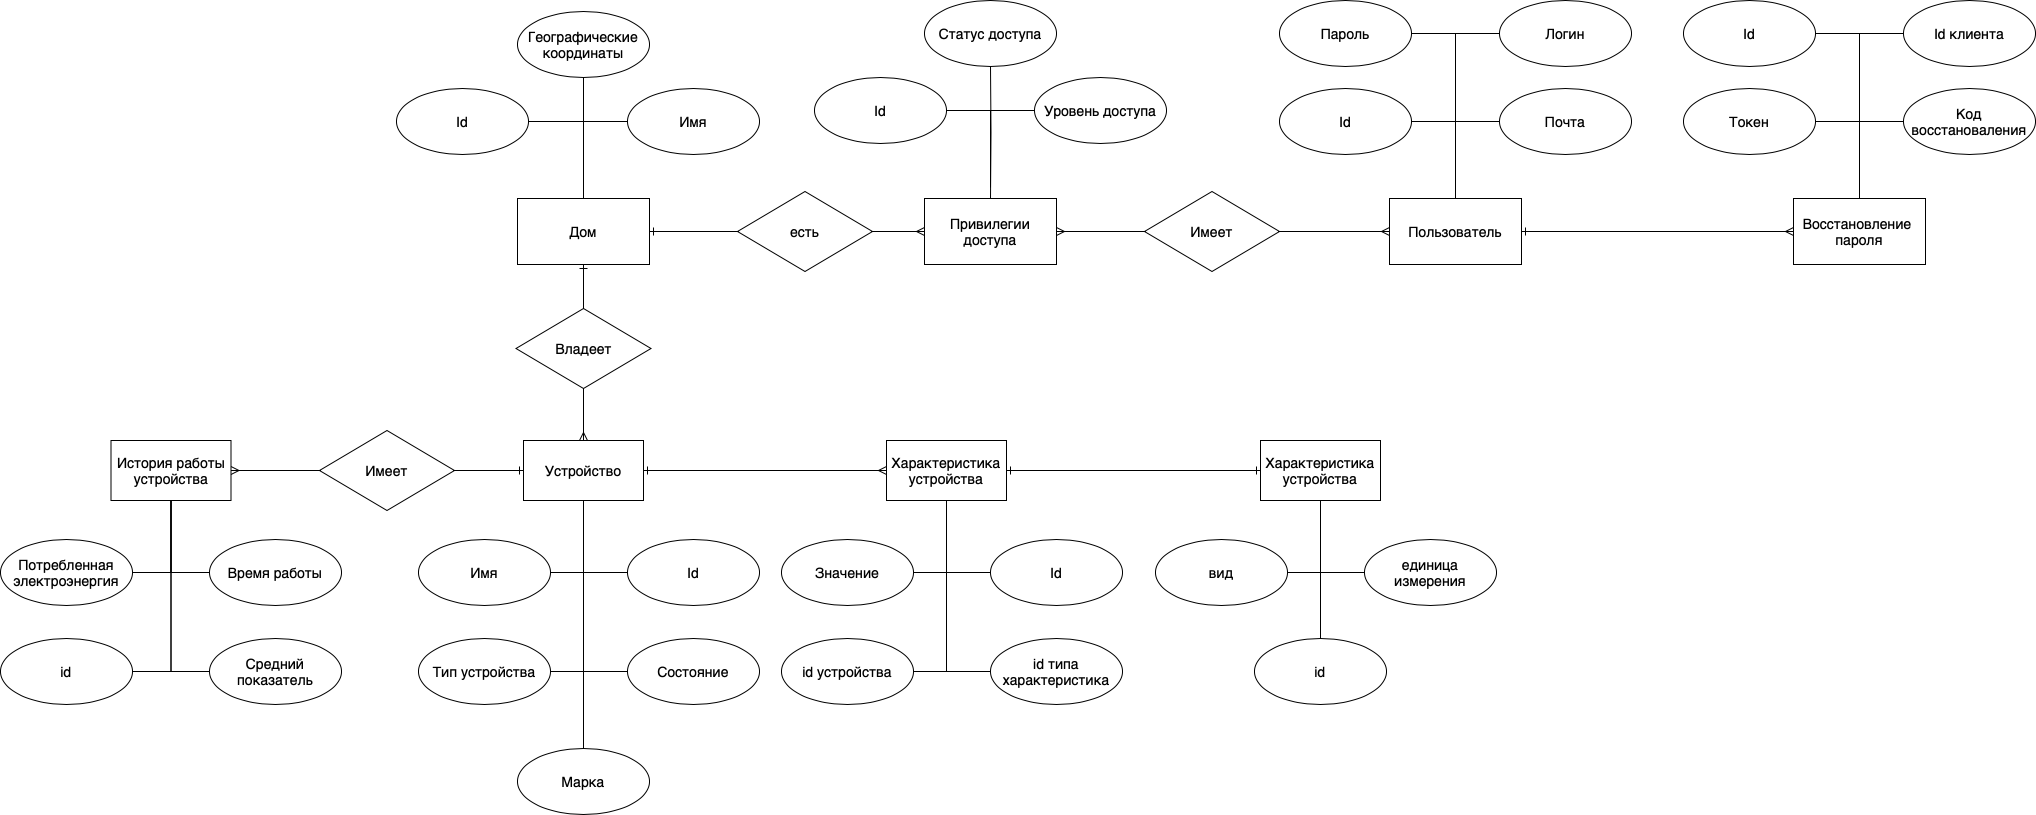
\includegraphics[width=1\linewidth]{img/er.png}
    \caption{ER-диаграмма в нотации Чена}
    \label{img:er}
\end{figure}
\noindent
\clearpage

\section{Формализация пользователей}

В зависимости от типа пользователя должен различаться набор доступных действий. Таким 
образом были выделены следующие категории пользователей:

\begin{enumerate}
    \item Гость -- пользователь, имеющий возможность 
    зарегистрироваться или авторизоваться на IoT-платформе умного дома.
    \item Авторизованный пользователь -- пользователь, который прошел авторизацию. 
    Он получает возможность создать собственный дом или присоединиться к уже существующему.
    \item Владелец дома -- пользователь, который создал дом. Ему доступны все возможные функции управления домом.
    \item Участник дома -- пользователь, который имеет доступ к дому другого пользователя. 
    Набор доступных действий определяет хозяин дома.
\end{enumerate}

Все доступные действия для каждой категории пользователей представлены на следующей Use-case диаграмме \ref{img:iot}
\begin{figure}[h]
    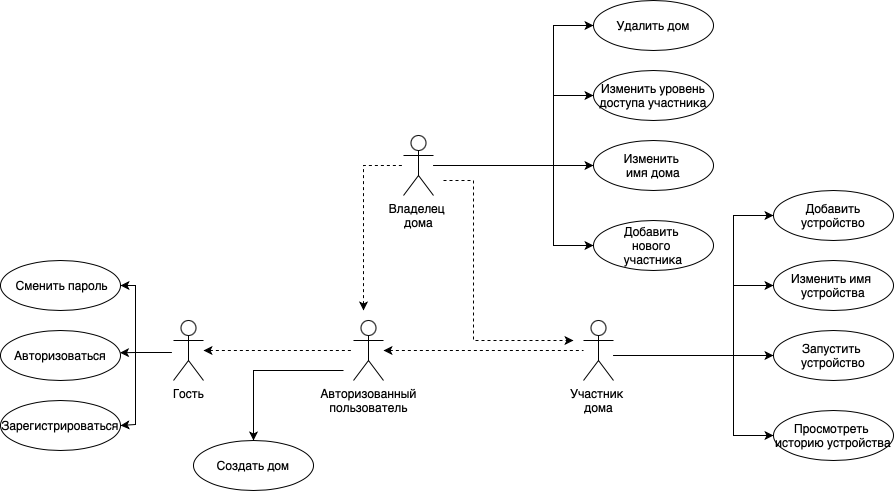
\includegraphics[width=0.9\linewidth]{img/ucd.png}
    \caption{Use-case диаграмм полльзователей}
    \label{img:iot}
\end{figure}
\clearpage

\section{Анализ существующих баз данных на основе формализации задачи}
База данных -- \textbf{самодокументированное} собрание \textbf{нтегрированных} записей \cite{kranke}. Рассмотрим части данного определения:
\begin{enumerate}
    \item База данных является самодокументированной, то есть содержит описание собственной струкутры, которое называется 
    словарем данных, каталогом данных или метаданными.
    \item База данных -- собрание интегрированных записей, она содержит:
    \begin{itemize}
        \item файлы данных,
        \item метаданные,
        \item индексы,
        \item может содеражть данные приложений.
    \end{itemize}
    \item База данных является информационной моделью пользовательской модели предметной области.
\end{enumerate}

Модель базы данных определяет логическую структуру базы данных и то, каким образом данные будут храниться, организовываться
и обрабатываться.

Существует три основных типа моделей базы данных:
\begin{itemize}
    \item дореляционные;
    \item реляционные;
    \item постреляционные.
\end{itemize}

\subsection{Дореляционная база данных}

К дореляционным моделям баз данных относятся иерархическая и сетевая модели.

Иерархическая модель состоит из объектов с указателями от родительских объектов к потомкам, 
соединяя вместе связанную информацию. Она может быть представлена в виде дерева. Одним из больших минусов данной
модели является невозможность отношения «многие-ко-многим».

Основными понятиями такой модели базы данных являюся узел и связь. Узел -- совокупность атрибутов данных, описывающих
некоторый объект. Данная база данных может быть предствлена в виде графа. При изменении структуры данной модели придется 
изменять и приложние, так как логика процедуры выборки данных зависит от физической организации этих данных~\cite{petr}.

\subsection{Реляционная база данных}
В реляционных моделях данные организованы в набор двумерных взаимосвязанных таблиц, 
каждая из которых представляет собой набор столбцов и строк, где столбец представляет атрибуты сущности, 
а строки представляют записи. Такое представление обеспечивает простой и эффективный способ хранения структурированной информации, 
доступа к ней, а также легкую сортировку.

Также в данной модели происходит разделение между физическим и логическим уровнями, что 
позволяет управлять физической системой хранения, не меняя данных, содержащихся в логической структуре~\cite{oracle}.

\subsection{Постреляционная база данных}

Постреляционная база данных -- это база данных, которая является расширенной версией реляционной 
модели базы данных и позволяет устранить ограничение неделимости данных, хранящихся 
в записях таблиц. Именно поэтому хранение данных в постреляционной модели по сравнению 
с реляционной считается более эффективным~\cite{fedor}.

Недостатком такой модели является сложность решения проблемы обеспечения целостности и непротиворечивости хранимых данных.~\cite{microsoft}.

\section*{Вывод}

В данном разделе проведен анализ аналогов IoT-платформ для умного дома.
Ни одно из исследованных решений не соответствовало всем установленным критериям сравнения. 
При рассмотрении моделей баз данных было принято решение в пользу реляционной модели. 
Это обосновано необходимостью обеспечения целостности хранящихся данных в разрабатываемой базе данных 
для IoT-платформы, а также простотой хранения структурированной информации и возможностью ее сортировки.

Кроме того, были формализованы поставленная задача, данные и категории пользователей.
